\documentclass[11pt]{article}
% =========================================================================
% SHARED STYLE FILE for 11_Master_Projects reports
% Visual style follows 0_Thesis_Submission/24m0553_AK_Gaurav_Mtech_Report.pdf:
% serif body font, blue hyperlinked TOC/links, ruled section headings,
% IITB-style title page, formal academic report structure.
% =========================================================================

\usepackage[a4paper,margin=1in]{geometry}
\usepackage{xcolor}
\usepackage{graphicx}
\graphicspath{{../images/}}
\usepackage{amsmath,amssymb}
\usepackage{booktabs}
\usepackage{caption}
\usepackage{float}
\usepackage[hidelinks]{hyperref}
\usepackage{titlesec}
\usepackage{enumitem}
\usepackage{setspace}
\usepackage[T1]{fontenc}
\usepackage{lmodern}
\usepackage{microtype}

% Every \includegraphics call is automatically framed with a thin black
% border (matches the printed look of figures/photos/charts in the source
% reports). \oldincludegraphics is kept available for institutional
% logos/seals on title pages, which should remain unframed.
\let\oldincludegraphics\includegraphics
\setlength{\fboxsep}{1pt}
\setlength{\fboxrule}{0.6pt}
\renewcommand{\includegraphics}[2][]{\fbox{\oldincludegraphics[#1]{#2}}}

\definecolor{thesisblue}{RGB}{0,0,205}
\hypersetup{
  colorlinks=true,
  linkcolor=thesisblue,
  urlcolor=thesisblue,
  citecolor=thesisblue,
  filecolor=thesisblue
}

\onehalfspacing
\setlength{\parskip}{6pt}
\setlength{\parindent}{0pt}

\titleformat{\section}
  {\normalfont\Large\bfseries}{\thesection}{1em}{}
\titleformat{\subsection}
  {\normalfont\large\bfseries}{\thesubsection}{1em}{}
\titleformat{\subsubsection}
  {\normalfont\normalsize\bfseries}{\thesubsubsection}{1em}{}

\newcommand{\reportTitlePage}[7]{%
  % #1 = Report title
  % #2 = Course code & name (e.g. "CE 605: Applied Statistics")
  % #3 = Subtitle/topic line (e.g. "Project Report 2: Network Analysis")
  % #4 = Author block (can be multi-line with \\ for group projects)
  % #5 = Supervisor name(s)
  % #6 = Programme line (e.g. "M.Tech in Transportation Systems Engineering")
  % #7 = Month/Year
  \begin{titlepage}
    \centering
    \vspace*{0.5cm}
    {\large\bfseries #2}\par
    \vspace{0.3cm}
    {\Large\bfseries #3}\par
    \vspace{1.2cm}
    {\Huge\bfseries #1}\par
    \vspace{1.5cm}
    \oldincludegraphics[width=3.2cm]{../../assets/iitb_logo.png}\par
    \vspace{1.2cm}
    Submitted by:\par
    \vspace{0.2cm}
    {\bfseries #4}\par
    \vspace{0.8cm}
    Under the Supervision of\par
    \vspace{0.2cm}
    {\bfseries #5}\par
    \vspace{1.2cm}
    #6\par
    Department of Civil Engineering\par
    \textbf{Indian Institute of Technology Bombay}\par
    Mumbai -- 400076, India\par
    \vspace{0.3cm}
    #7\par
  \end{titlepage}
}

\newcommand{\reportAbstract}[1]{%
  \section*{Abstract}
  #1
  \vspace{0.5cm}
}


\title{Mobility Ecology of Thane Railway Station}
\author{Abhijeet Kumar Gaurav}
\date{}

\begin{document}

\reportTitlePage
  {Mobility Ecology of Thane Railway Station}
  {PS 651: Mobility Policy and Infrastructure}
  {Project Report: Mobility Ecology of Thane Railway Station}
  {Abhijeet Kumar Gaurav (24M0553)}
  {Course Instructor, PS 651}
  {M.Tech in Transportation Systems Engineering}
  {Spring 2025}

\pagenumbering{roman}

\reportAbstract{
Thane Railway Station, the busiest suburban station on Mumbai's Central Railway and the
interchange between the Central main line and the Trans-Harbour line, handles approximately
6--7 lakh (600,000--700,000) passengers and over 1,000 trains daily across ten platforms. This
study examines Thane station as a dynamic \textit{mobility ecosystem} rather than a mere transit
point, applying a Hardware--Software--Practice framework to three tightly interdependent
operational systems: the Passenger Management System, the Emergency Response \& Disaster
Management System, and the Technology \& Digital Integration System. For each system, the
station's physical infrastructure (hardware), its institutional rules and operational policies
(software), and the observed real-world commuter and staff behaviour (practice) are analysed in
turn, drawing on a Station Manager interview, field observation, and secondary news and
policy sources. A focused pedestrian mobility analysis of the West Entry, covering the
ground-level TMT bus/auto-stand access, the first-deck skywalk entry, and their merge at the
dome staircase leading to Platform~1, identifies three critical conflict zones associated with
entry bottlenecks, reverse flow collisions, and high-density stampede risk. The station is
further situated within Thane city's broader urban and governance ecosystem, including the
SATIS-West and SATIS-East multi-modal redevelopment projects, upcoming Metro Line~4
integration, and the shared jurisdiction of Indian Railways, the Thane Municipal Corporation,
RPF, and GRP. The study concludes that Thane functions as an interdependent system of systems
operating near capacity, where good passenger-flow design directly reduces emergency risk, and
recommends a comprehensive crowd management plan, enhanced emergency preparedness (security
screening, 24/7 medical cover), and continued technology leverage (AI-based crowd density
monitoring, unified ticketing) to sustain Thane as a safe, accessible, people-centric mobility
hub.

\vspace{0.3cm}
\noindent\textbf{Keywords:} Mobility Ecology; Railway Station Design; Passenger Management;
Crowd Management; Emergency and Disaster Management; Digital Integration; Pedestrian Conflict
Analysis; Multi-Modal Integration; Thane Railway Station
}

\newpage
\tableofcontents
\newpage
\pagenumbering{arabic}

\section{Introduction and Context}

Thane Railway Station is one of the busiest transit hubs in India, serving as a crucial node in
the Mumbai Metropolitan Region's suburban railway network. Historically, Thane was the
destination of India's first passenger train in 1853, and today it remains a people-centric
mobility hub integrating multiple transport modes. The station handles approximately
6--7~lakh (600,000--700,000) passengers daily, with over 1,000 trains, including roughly
55--60 long-distance expresses, passing through its 10~platforms each day. Thane's unique
position as the interchange between Central Railway's main lines and the Trans-Harbour line
means it not only funnels commuter traffic between Mumbai and its suburbs but also connects to
Navi Mumbai and beyond. The station's design and operations thus directly impact the
accessibility, safety, comfort, and integration of mobility for hundreds of thousands of daily
travellers.

\begin{figure}[H]
\centering
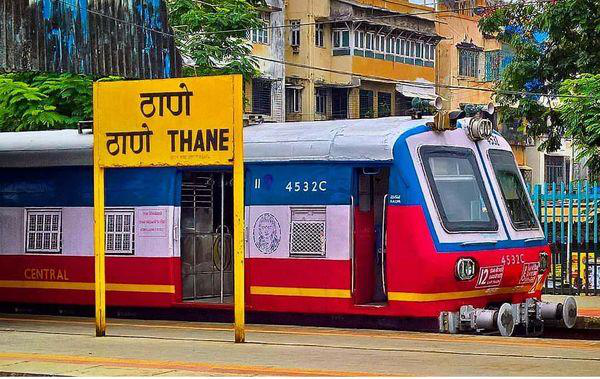
\includegraphics[width=0.55\textwidth]{fig_station_photo.png}
\caption{Thane Railway Station.}
\end{figure}

\begin{figure}[H]
\centering
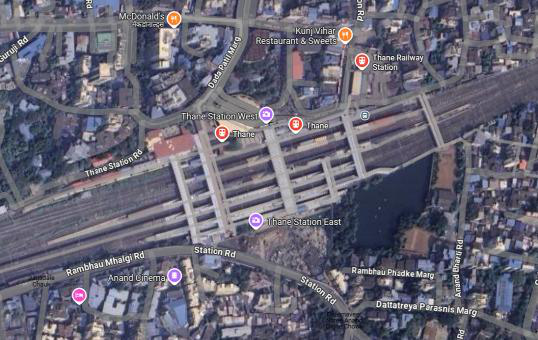
\includegraphics[width=0.6\textwidth]{fig_map_aerial.png}
\caption{Aerial (Google Maps) view of Thane Station and its surrounding road network.}
\end{figure}

\section{Objectives and Methodology}

This study investigates Thane Railway Station as a dynamic ecosystem of mobility, rather than a
mere transit point. Adopting a \textbf{Mobility Ecology Framework}, the research focuses on
three core operational systems, namely the Passenger Management System, the Emergency Response \&
Disaster Management System, and the Technology \& Digital Integration System, and analyses
how these systems interact with one another and with commuter behaviour. Using the
\textbf{Hardware--Software--Practice model}, the study explores the real-time functioning of the
station and its embeddedness in Thane city's larger urban transport and governance fabric.

The core objectives of the study are to:
\begin{itemize}
  \item Analyse Thane Station's mobility systems using the Hardware--Software--Practice model,
  where \textbf{Hardware} denotes physical infrastructure and tools, \textbf{Software} denotes
  institutional rules, operational policies, and management practices, and \textbf{Practice}
  denotes commuter behaviour, decision-making, and real-world flow patterns;
  \item Understand how infrastructure (hardware) is governed by policy systems (software), and
  how both are influenced by commuter practice;
  \item Examine the interactions and dependencies between passenger flow management, emergency
  handling protocols, and digital systems such as CCTV, public-address systems, and ticketing
  apps;
  \item Evaluate how Thane Station integrates into urban infrastructure, particularly the bus
  terminals, auto stands, skywalks, and road access on either side of the station, the
  SATIS-West and SATIS-East projects by the Thane Municipal Corporation (TMC) and Indian
  Railways, and the upcoming Metro Line~4 integration and commercial transit nodes.
\end{itemize}

The study draws on a Station Manager interview, direct field observation of pedestrian and
vehicular flow (particularly at the West Entry), and secondary sources including news reports
and municipal planning documents (full list in the References section).

\section{System Overview}

Thane Station operates as a system of systems. Fourteen identified subsystems, from ticketing
and security to sanitation and freight, together constitute its Governance \& Administrative
System. This report focuses on the three subsystems that most directly shape the daily
commuter experience:
\begin{enumerate}
  \item \textbf{Passenger Management System:} how passengers move, wait, and board trains;
  \item \textbf{Emergency \& Disaster Response System:} how the station handles unexpected
  events;
  \item \textbf{Technology \& Digital Integration System:} how digital tools assist operations
  and users.
\end{enumerate}

\begin{figure}[H]
\centering
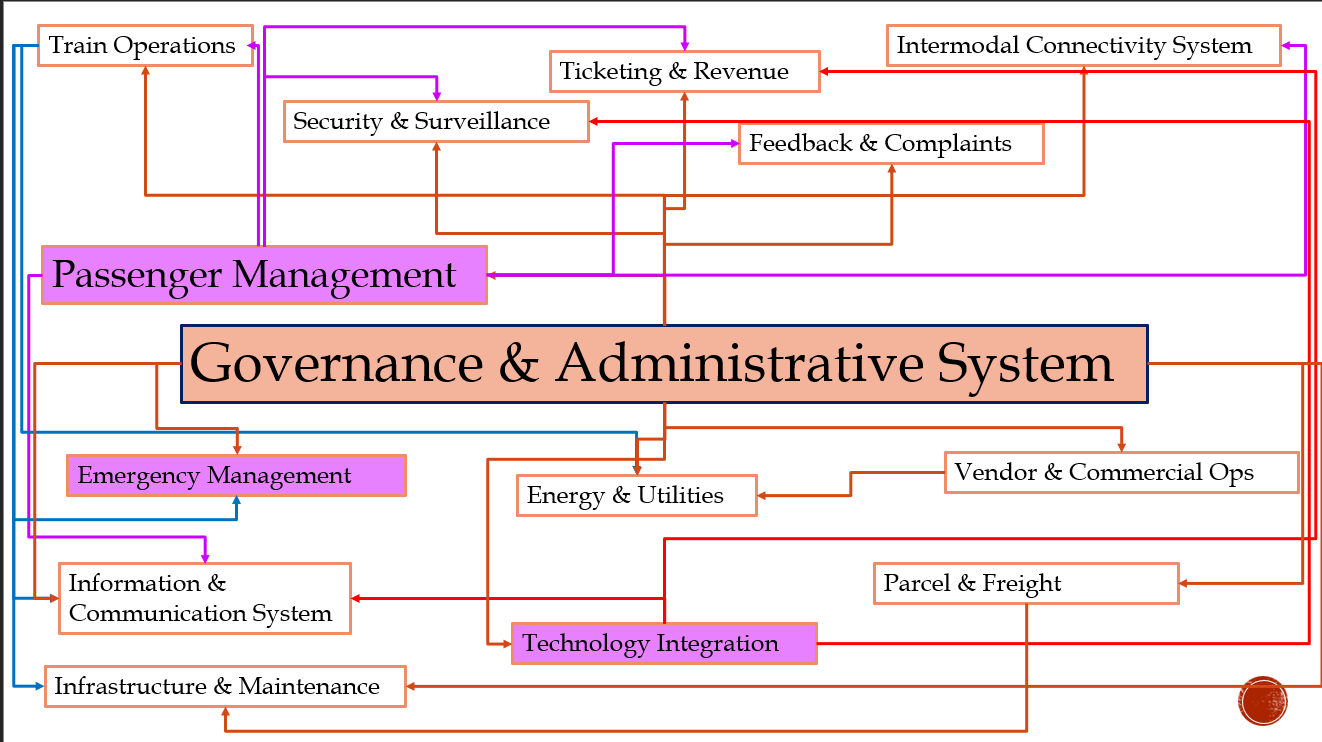
\includegraphics[width=0.85\textwidth]{fig_system_diagram.png}
\caption{Probable system diagram of Thane Station, showing the Governance \& Administrative
System and its interconnected subsystems.}
\end{figure}

These three systems were chosen because they collectively shape daily commuter movement,
mitigate emergencies, and optimise station operations. A breakdown in any one of these systems
can disrupt the entire network; for example, a digital failure such as a missed platform
announcement can quickly escalate into passenger confusion and panic.

\section{Passenger Management System}

The Passenger Management System at Thane encompasses all aspects of handling the enormous flow
of commuters, from station design and facilities to operational strategies and crowd control
measures to the actual patterns of passenger movement and behaviour. Effective passenger
management is critical for accessibility (ease of use for all travellers), safety (preventing
overcrowding hazards), and comfort (providing a pleasant transit experience).

\subsection{Hardware: Infrastructure for Passenger Flow}

Thane station has two main entrances/exits, \textbf{Thane West} and \textbf{Thane East},
connected by multiple Foot Over Bridges (FOBs). The West side is the busier, more developed
entry, uniquely structured on two levels: a ground-level entrance aligned with an auto-rickshaw
stand, and an upper-level entrance connected to a bus terminus (the TMT bus depot). Commuters
arriving by bus can directly enter the station's first-floor concourse from a dome-shaped depot
structure, buy tickets at an upper-level ticket counter, and access the FOBs without descending
to ground level. Likewise, a system of skywalks on the west side feeds pedestrians into the
station's first-floor entry from surrounding roads. These integrated walkways and decks have
made the west side a thriving interchange zone, contributing to significantly higher footfall
on the west relative to the east. In contrast, the Thane East side is currently undergoing major
construction (as part of SATIS-East), with relatively lower footfall due to ongoing works. A
newly built road overbridge (Kopri Bridge/Koliwada New Bridge) now links Thane East and West for
general traffic without funnelling people through the station, helping segregate through-traffic
from station crowds.

\begin{figure}[H]
\centering
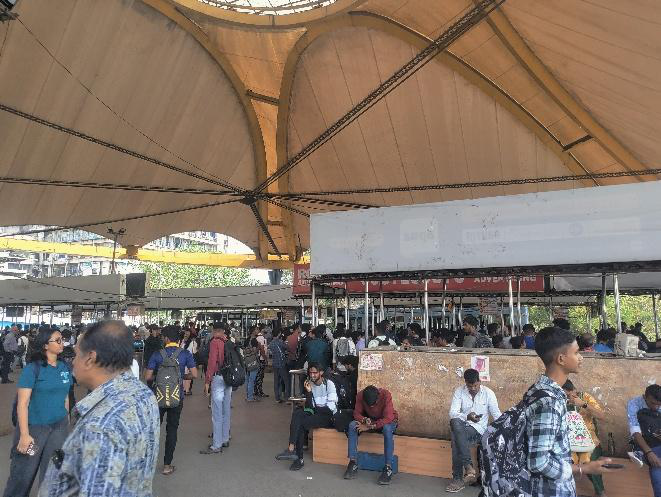
\includegraphics[width=0.85\textwidth]{fig_bus_stand_deck.png}
\caption{Bus stand on the first floor of Thane Station.}
\end{figure}

Thane's 10 platforms are long (around 300~m), accommodating 12--15-coach suburban and
long-distance trains. Platforms~1--5 primarily serve slow and fast suburban trains on the
Central line, while Platforms~6--10 handle suburban trains and some long-distance trains. As of
early 2024, six FOBs connect all platforms and often extend to both the East and West exits. Two
new FOBs were opened in 2024: one at the station's Mumbai end (north), 130~m long and 5.5~m
wide, and another at the Kalyan end (south), 76~m long and 4.8~m wide, built jointly by Central
Railway and TMC after older skywalks were declared unsafe and demolished in 2019. The increase to
six FOBs is directly aimed at relieving congestion and distributing passenger load more evenly,
as previously only four bridges led to severe chokepoints during rush hours. The FOBs allow
passengers to move between platforms without crossing tracks and also serve as east--west
connectors for local residents, essentially acting as public footpaths over the railway. Despite
the huge crowds, the presence of multiple FOBs has been noted to somewhat ease movement by
providing alternate routes; however, their effectiveness continues to depend on sufficient width
and strategic entry/exit design.

The station also has designated staircases on each platform, though these often overflow with
people during peak hours. Notably, the station currently lacks any dedicated ramps for
wheelchair users; this absence, combined with occasional elevator outages or overcrowding, poses
challenges for differently-abled passengers despite Thane being a major hub.

\begin{figure}[H]
\centering
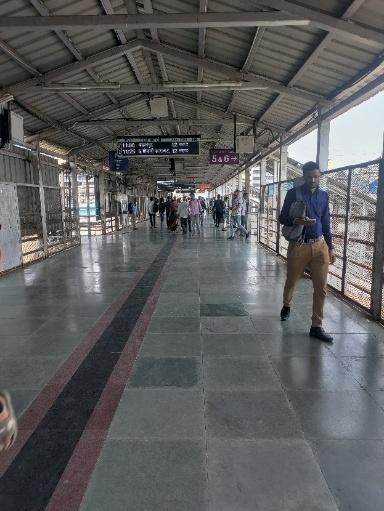
\includegraphics[width=0.45\textwidth]{fig_new_fob.png}
\caption{Interior of a new FOB at Thane, connecting platforms above track level.}
\end{figure}

On the concourse and platform level, other hardware elements include ticketing facilities
(several ticket booking counters and 25 Automatic Ticket Vending Machines for unreserved
tickets), electronic information displays, public address speakers, CCTV cameras, and amenities
such as seating, drinking water, restrooms, and first-aid rooms. Parking facilities are
available: a dedicated area on the first floor for two-wheelers and space for four-wheelers on
the east side, though these often overflow at peak times. The station's infrastructure is thus
extensive and multi-layered, designed to channel massive pedestrian flows efficiently.

\begin{figure}[H]
\centering
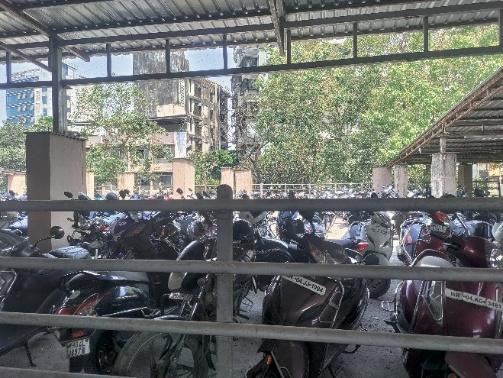
\includegraphics[width=0.75\textwidth]{fig_parking.png}
\caption{On-street and off-street two-wheeler parking at Thane Station.}
\end{figure}

Despite these facilities, certain hardware limitations at Thane contribute to crowding issues.
The station does not have segregated entry and exit gates: most footbridges and concourse
passages are bi-directional for incoming and outgoing passengers. Passengers essentially exit
through the same gates they enter, creating cross-flows that intensify congestion. This design
makes the station sensitive to stampede-like situations during peak times, since opposing
streams of people must negotiate limited space. Additionally, security infrastructure is
minimal: there are no permanent baggage scanners or metal detector door-frames at entrances,
which, while intended to streamline movement, also raises safety concerns. The hardware of
Thane station thus presents a mixed picture: a large-scale, complex infrastructure that has been
steadily augmented (new bridges, escalators, etc.) to handle rising demand, yet still strained
by sheer volume and some design drawbacks.

\subsection{Software: Policies, Management, and Institutional Setup}

The software component of passenger management refers to the rules, protocols, and management
strategies that govern how passengers use the station. At Thane, multiple agencies and policies
intersect to maintain order: Indian Railways (Central Railway's Mumbai division) operates train
services and station facilities, the Station Manager's office and booking staff handle ticketing
and announcements, and the Railway Protection Force (RPF) and Government Railway Police (GRP)
handle crowd control and security.

\textbf{Operational policies and scheduling.} Thane station operates virtually round-the-clock,
with first local trains around 4~AM and the last past midnight, plus long-distance trains at
various hours. Peak commuting hours are 7--11~AM (morning inbound) and 5--10~PM (evening
outbound) on weekdays, during which train frequency on the Central line is exceptionally high.
Despite this, peak periods see severe crowding on platforms and FOBs as thousands attempt to
board or exit simultaneously. Central Railway schedules ``mega blocks'' (maintenance blocks) on
weekends or off-peak times to upgrade tracks; roughly 55--60 long-distance trains halt at
Thane, requiring coordination of platform usage between fast locals and express trains.

\textbf{Staffing and crowd control measures.} RPF personnel and railway staff are deployed at
key crowd-pressure points, for instance at the stairways of busy FOBs and on Platforms~9/10,
which serve the Trans-Harbour line and see acute overcrowding. During the heaviest rush, extra
ticket collectors may also help channel passenger flows and discourage fare evasion. However,
commuters report that staffing is insufficient for the size of the crowd, and an RPF official
has acknowledged that more staff are needed to manage the increasing crowd. In practice, much
crowd control is reactive: if a platform becomes dangerously packed, RPF may temporarily hold
people at the concourse or regulate flow on a footbridge, but on regular days formal queuing or
one-way routing is not enforced on the bridges or stairs, leading to chaotic free-for-all
movement.

\textbf{Queue systems and passenger guidance.} Recognising the chronic congestion, authorities
have experimented with queue systems for boarding trains. In early 2018, Central Railway
introduced a pilot ``queue for ladies'' initiative at Thane and other major stations, where women
commuters, especially for ladies-only compartments, were encouraged to form lines on marked
platform areas. This has met with some success, though implementation remains mainly limited to
ladies' and sometimes first-class coaches, and is not universally followed in general
compartments. Aside from platform queues, other soft measures include platform markings, signage
instructing passengers to exit before boarding, and periodic public announcements urging caution
and patience. The Station Manager's team monitors peak crowding and can request additional train
halts or initiate empty trains from Thane to clear the rush.

\textbf{Institutional coordination.} Management of Thane's passenger flows is supported by
higher-level planning and coordination. Thane is classified as an ``NSG-1'' (Non-Suburban
Grade-1) category station, meaning it is among the top revenue and footfall generators and thus
gets priority for upgrades. The Mumbai Railway Vikas Corporation (MRVC) has conducted passenger
counts and recommended decongestion projects at Thane as part of the Mumbai Urban Transport
Project. The Thane Municipal Corporation, while not managing railway operations, plays a role
through SATIS projects that create dedicated spaces for feeder buses and autos. Passenger
associations (commuter advocacy groups) at Thane have repeatedly pressed for better crowd
management, including demands for more frequent train services, more FOBs, and enforcement of
line systems, indicating a governance dimension where policy changes are needed to
sustainably manage crowds beyond what station staff alone can handle.

\subsection{Practice: Passenger Behaviour and Flow Patterns}

Intense crowding, routinised behaviours by commuters, and occasional order breakdowns during
daily operations characterise Thane Station's real-world practice.

\textbf{Peak-hour crowds.} During rush hours, Thane station sees stampede-like crowd densities
on its footbridges, staircases, and platforms; commuters often describe the experience as
``completely chaotic.'' A regular traveller recounted that it can take 15--20~minutes to exit
the station after alighting in the evening, due to the slow-moving throng on narrow bridges. In
these conditions, personal space is minimal and pushing and jostling become the norm. Commuters
have adapted coping behaviours: timing their exit by choosing less-crowded FOBs, using the
longer West-side skywalk route that disperses crowds better, or waiting on the platform until
the initial rush clears. Despite such strategies, at peak volume the infrastructure often runs
at or beyond capacity. Commuters have expressed genuine fear that a stampede might occur at
Thane station due to inadequate crowd management, invoking memory of the deadly 2017
Elphinstone Road station stampede in Mumbai.

\textbf{Daily routines and social norms.} Within the bustling environment, unwritten social
norms have evolved: boarding/alighting etiquette where most passengers allow those on the train
to alight first before boarding; a two-line queue before the train arrives, especially in
first-class and ladies' sections, though crowd pressure often overwhelms orderly boarding in
general compartments; ``return-journey'' seat securing, where some commuters ride a train one
stop in the opposite direction to secure a seat for the long ride, circumventing the queue
system; and, on footbridges, no fixed keep-left/keep-right convention, so one side of a bridge
may occasionally be taken over by a predominant flow, forcing opposite movers to squeeze
through. Compliance with formal rules is mixed: while most use footbridges properly, a few risk
crossing tracks in desperation if platforms are too packed, though RPF fines offenders when
caught.

\textbf{Accessibility and user experience.} Elderly and differently-abled passengers often
struggle in the crowd; without ramps, wheelchair users or those who cannot climb stairs must use
elevators, which can be difficult to reach through a sea of people. Women commuters have voiced
both positives (ladies' queues, presence of women RPF constables improving safety and comfort)
and negatives (harassment or groping still occurring in packed mixed-gender crowds on bridges).
Night-time travel (post 10~PM) sees thinner crowds, alleviating congestion but raising personal
safety concerns, though Thane's premises are well-lit and continuously monitored. Perception of
safety strongly shapes commuter behaviour: people tend to avoid isolated stretches of platform
and prefer staying with the crowd, which ironically exacerbates crowding. Many Thane commuters
have adapted with a resilient mindset, expecting delays and pushiness and budgeting extra
time.

\textbf{Interplay with other modes.} Every weekday morning, waves of commuters pour off trains
and head to the TMT buses, BEST/NMMT buses, or the auto-rickshaw queue on the West side, timing
their arrival to catch a specific bus or fast local, a coordinated dance between train and bus
schedules that regulars master. The lack of an organised pick-up/drop-off zone on the East
(pending SATIS-East completion) means passengers habitually prefer the West for its convenient
onward transport options, a behavioural imbalance that the new east-side development aims to
correct.

In summary, practice at Thane station is one of high-density, kinetic movement that is both
adaptive (commuters finding ways to cope and cooperate) and at times hazardous (bottlenecks that
can spark dangerous situations). The evidence suggests that while the station manages to move
an enormous number of people, it operates very much at the limits of its capacity, requiring
urgent improvements and continuous management vigilance.

\section{Emergency Response \& Disaster Management System}

With such intense daily usage, Thane Railway Station is prone to routine overcrowding,
emergency situations, and potential disasters, ranging from accidental falls, medical
emergencies, and small fires to larger-scale crises like stampedes, train derailments, or
security threats. The station's Emergency Response \& Disaster Management System is therefore a
critical aspect of its mobility ecology, directly tied to passenger safety.

\subsection{Hardware: On-Site Emergency Infrastructure}

\textbf{Fire safety equipment.} Given the fire risk in a busy station (from electrical short
circuits, discarded cigarettes, etc.), Thane has installed basic firefighting hardware: portable
fire extinguishers suitable for different fire classes are placed on platforms and concourses,
water hose points are connected to the station's water supply, and sand or mud is stored on-site
to smother fires. However, no dedicated fire brigade unit is stationed at Thane, so the station
relies on calling city fire services for significant fires. A March~2025 fire incident, dry
waste on a platform roof catching fire, illustrates the hardware and response: station
authorities immediately cut power to the overhead electric lines and summoned the Thane
Municipal Corporation's fire rescue team, who doused the flames within minutes. The quick
isolation of electrical supply via trackside circuit breakers is a critical hardware capability
in electrified rail systems during fire emergencies. Overall, while basic firefighting tools
exist, the station lacks more advanced systems such as automatic fire detection or sprinklers,
relying on human vigilance and portable equipment.

\textbf{Medical facilities and equipment.} Thane station has a First Aid Room / Emergency
Medical Room (EMR) on Platform~2, set up through a public--private partnership with a local
hospital, equipped in principle with a stretcher and basic life-saving supplies and meant to be
staffed by doctors or paramedics. In practice, the Station Manager noted that medical services
are unavailable during night hours, implying the EMR is staffed mainly in the daytime. During
the day, the EMR treats minor injuries and cases of giddiness, with serious treatment free for
railway accident victims. The station also keeps stretcher trolleys and wheelchairs handy, and
RPF personnel are trained to use them; for more serious emergencies, an ambulance can be called
from Bhanushali Hospital (about 1~km away) or the civil hospital, given Thane's dense urban
setting with multiple hospitals within a few minutes' drive.

\textbf{Crowd and disaster management tools.} Unlike a building with defined emergency exits, a
railway station's emergency egress routes are essentially the same as its normal ones, namely the
footbridges, staircases, and station roads, so Thane's lack of separate entry/exit routes is
also a hardware shortcoming in disaster scenarios. Authorities do have physical tools for crowd
management, including steel barricades and ropes to block off passages or create guided lanes,
and designated holding areas (e.g., the bus depot deck) where crowds can be redirected. CCTV
cameras throughout the station, while primarily a security tool, also serve as an early warning
system for detecting developing hazards. Staff carry wireless radios and hotline phones
connecting the station control to railway headquarters and city emergency services, and
platforms and FOBs are well-lit with backup generators on standby. For rail-specific accidents,
Central Railway maintains Accident Relief Medical Vans and breakdown cranes at nearby locations
such as Kurla and Kalyan.

\subsection{Software: Protocols, Roles, and Coordination}

\textbf{Emergency protocols and chain of command.} Thane follows standard Indian Railways
disaster management protocols specifying the roles of officials during emergencies. The Station
Manager is usually the incident commander on-site until higher authorities arrive, able to order
power off on affected tracks and inform the Divisional Control Office. The Safety Department of
the railway oversees fire preparedness, while actual firefighting at Thane is locally managed by
RPF under that department's guidance. For medical emergencies, the Station Master, with RPF's
help, manages the situation. If an incident escalates (multiple injuries, a large brawl), the
GRP is called in to take charge of law and order, working closely with RPF.

\textbf{Stampede and crowd disaster management.} Given the ever-present risk of stampedes, the
immediate protocol if a stampede-like situation starts is for RPF and GRP to physically
intervene: forming human barriers, diverting the route, and blocking FOBs to stop the access
load, possibly re-routing people to another footbridge. Importantly, policy dictates that public
announcements are \emph{not} made in the initial stage of such an emergency, to avoid causing
panic that could worsen the stampede; the practice is to quietly and swiftly manage the crowd
until the situation is under control, then make informative announcements. Additionally,
Thane's RPF and GRP, along with city police, periodically conduct mock drills for scenarios such
as bomb threats or evacuation, internalising lessons from the 2017 Elphinstone stampede.

\textbf{Security threat response.} In the event of a security threat, Thane's protocols involve
rapid coordination with specialised units. When a suspicious unattended bag was spotted near the
station in 2018, local police and the bomb squad were alerted immediately, cordoned off the
area, and cleared bystanders before the bomb disposal squad inspected the bag, which turned out
to be a false alarm. Typically the GRP leads station security threats, working with Mumbai
Police's Anti-Terror units if needed. Since Thane currently lacks metal detectors and X-ray
scanners at entry points, the software side compensates through intelligence and vigilance --
RPF officers watch for suspicious behaviour, and announcements remind passengers to report
unclaimed objects.

\textbf{Disaster management planning and governance.} Thane station's disaster management is
part of the city and regional disaster planning: the Thane Municipal Corporation's Disaster Cell
is involved in events like major fires or building collapses nearby, and the Railway's Divisional
Disaster Management Plan allocates resources such that, within minutes of a significant accident,
medical and rescue teams from nearby stations (Mulund, Dombivli) would rush to the site.
Emergency contact numbers (Railway helpline 182 for security, 108 for ambulance) are displayed,
regular training is given to station staff on first aid and emergency communication, and the
station collaborates with NGOs such as Railway Commuter Safety groups and St.\ John's Ambulance.
The cooperative replacement of unsafe FOBs after 2019, requiring both political intervention
and municipal funding, illustrates this multi-layered governance in action. One notable gap
remains the absence of preventive security checks, which the railway plans to eventually address
with metal detectors and baggage scanners at major stations including Thane.

\subsection{Practice: Handling Real Emergencies on the Ground}

Despite the challenges, several real incidents illustrate how Thane's emergency systems have
been tested in practice.

\textbf{Fire incident, March 2025:} a small fire on a platform roof, caused by dry debris, was
swiftly handled: a motorman noticed smoke and reported it, station authorities cut traction
power, trains were halted for about 8--9~minutes, and fire services were called. Commuters were
moved away from the affected end of the platform calmly, and service resumed within minutes,
demonstrating good coordination between railway staff and city emergency responders.

\textbf{Bomb scare, 2018:} the practice of evacuation and search was implemented well: police
cordoned the immediate area and had nearby shops shut to reduce onlookers, avoiding panic; no
stampede occurred even though the scare took place near the station during morning hours, and
trains continued running as the affected area was outside the platforms.

\textbf{Medical emergencies:} these are common at Thane, ranging from commuters feeling faint to
minor injuries while boarding. A case noted in 2015 recorded that, within a day of the EMR
opening, it treated four cases of heat-induced giddiness and a leg injury. Usually RPF or other
passengers help bring the person to the first-aid room, and trains have occasionally been
delayed a few minutes to accommodate transferring a sick passenger to an ambulance. A recognised
gap is the night-time medical service window: if a medical emergency occurs at, say, 2~AM, the
protocol relies on co-passengers and whatever first-aid training railway staff have until a city
ambulance arrives, an area identified for improvement (ensuring 24/7 medical attendants).

\textbf{Monsoon flooding and disruptions:} although Thane station is relatively elevated and
thus less flood-prone than some other stations, heavy Mumbai monsoons still test the system.
Waterlogged tracks or a flooded rail underpass can cause train delays that lead to platform
overcrowding, in practice an effective crowd-management emergency in its own right. RPF and
station staff manage such situations through continuous announcements about delays, opening
additional exits to disperse crowds, and liaising with TMC on road traffic outside. During
severe disruptions, the station has also served as a shelter for stranded passengers, with rail
personnel distributing water or arranging buses.

Overall, the pattern is that small-to-medium incidents at Thane are handled decently through
staff initiative and external coordination, though the station remains vulnerable to a
large-scale disaster given the sheer footfall. The interconnection between passenger management
and emergency management is evident: good passenger-flow design directly reduces emergency
risk, while emergency preparedness such as drills and clear protocols can save lives in the
critical moments when the hardware and practice of normal operations come under stress.

\section{Technology \& Digital Integration System}

Thane Station's Technology \& Digital Integration System is increasingly important in enhancing
efficiency, safety, and user experience in an era of smart infrastructure. This system covers the
digital and electrical systems that support station operations and passenger services, from
signalling and train control tech to commuter-facing apps and information systems, and involves
integrating the station's operations with broader digital networks.

\subsection{Hardware: Digital and Electronic Infrastructure}

Thane is a key node in Central Railway's signalling network, with a centralised electronic
interlocking system, managed by the Signal \& Telecom (S\&T) Department, governing all train
movements through the station and enabling over a thousand daily train services to be routed
safely between the fast, slow, and Trans-Harbour lines. The station has a network of CCTV
cameras covering platforms, footbridges, and entry/exit points, feeding into a local monitoring
room typically manned by RPF as part of Indian Railways' Integrated Security System; the cameras
act as a crime deterrent and allow rapid identification of incidents such as a person falling on
the track. Passenger information systems include LED indicator boards on each platform and
larger electronic boards at entrances listing upcoming trains, synchronised with the railway's
scheduling system, along with automated multi-language announcement systems broadcast through a
station-wide loudspeaker network.

\begin{figure}[H]
\centering
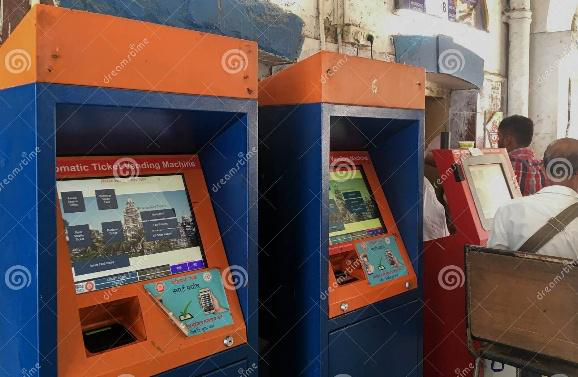
\includegraphics[width=0.45\textwidth]{fig_atvm.png}
\caption{Automatic Ticket Vending Machines (ATVMs) at Thane Station.}
\end{figure}

For ticketing and entry, Thane has 25 Automatic Ticket Vending Machines (ATVMs) as touchscreen
kiosks for suburban tickets via smart card or coins, handheld Ticket Checking Devices for TCs,
and QR-code scanners for mobile-app tickets purchased through the UTS (Unreserved Ticketing
System) app. Free public Wi-Fi, installed as part of RailWire/RailTel's initiative at
A-category stations, and mobile charging points on platforms round out the digital-era
amenities. Looking ahead, the SATIS-East project and the planned 11-storey station complex may
bring a centralised control centre, more advanced surveillance, better integration with city
traffic control, integrated multi-modal ticketing, and rooftop solar panels.

\subsection{Software: Digital Systems Management and Integration}

The Central Railway Information Systems (CRIS), the IT arm of Indian Railways, manages
applications such as the UTS mobile app and back-end databases; ticketing data at Thane feeds
into the UTS backend so that a paperless mobile ticket can be validated on demand by RPF or TC.
CRIS also manages the Passenger Reservation System for long-distance tickets, digitally
integrating Thane with the broader railway network's schedules and reservation updates.
CCTV feeds are plausibly linked to basic motion-sensing video analytics, and the public
announcement software is programmed to trigger multi-language announcements automatically as a
train approaches a signalling block, with manual override available to the Station Master.

As part of Thane Smart City initiatives, an Intelligent Transport System (ITS) by TMC aims to
incorporate train arrival information into bus-departure adjustments, and the Smart City project
envisions city-wide CCTV including the station road. Third-party apps such as M-Indicator,
though not railway software, are heavily integrated into commuters' daily experience. On
ticketing and fare integration, the UTS app supports season-pass booking and GPS-geofenced
paperless tickets that must be activated within range of the station to prevent misuse, and
ATVM smart cards can now be recharged via the app. On security software, the RPF likely uses the
Railway Security Management System to log incidents and coordinate with the central RPF control
room at Mumbai CST. Institutionally, ``Digital India'' policy has pushed the station toward
e-tools, namely digital payment options, mobile ticketing, and free Wi-Fi, while the S\&T
Department maintains the underlying tech and RPF/station staff operate it day to day. A key
challenge remains ensuring real-time responsiveness: no software can fully predict sudden crowd
surges, so human decision-making remains crucial even as digital data increasingly informs
better operational decisions.

\subsection{Practice: Impact of Technology on Passengers and Operations}

Thane's commuters are increasingly tech-savvy: a growing number use the UTS mobile app to book
tickets and avoid queuing altogether, gradually reducing crowding at ticket windows and ATVMs,
though uptake remains moderate as many still prefer physical tickets or season passes. Many
passengers also use apps like M-Indicator or the official Railways app to check schedules and
real-time delays, aided by free station Wi-Fi; this digital awareness helps commuters make quick
decisions and has empowered them to report crowd conditions or faults via social media, which
railway authorities monitor as a new facet of participatory problem-solving.

Technology has produced tangible efficiency gains: automated multi-language announcements ensure
prompt information even when staff are occupied, digital displays offer instant route
confidence, CCTV surveillance has helped RPF spot incidents such as petty theft faster, and
modern signalling has increased throughput by enabling closely spaced train operations. However,
not all integration is smooth: occasional display or announcement-system glitches can sow
confusion, a digital divide persists among elderly passengers less comfortable with apps or
ATVMs, and CCTV remains fundamentally reactive rather than preventive in the absence of entry
screening; in dense crowds, cell networks can also become congested. Staff practice has adapted
accordingly: ticket clerks now handle more digital customer-service queries, RPF personnel
monitor CCTV feeds as part of their daily duty, and the Station Manager uses a computer
dashboard to track train movements and crowd levels. The COVID-19 pandemic accelerated this
shift concretely: post-lockdown, heavy promotion of the UTS app for contactless ticketing saw
constant growth in adoption, benefiting a major station like Thane by helping maintain
distancing at counters, an integration that has remained useful even after normalcy returned.

In conclusion, technology at Thane station serves as a force multiplier for both efficiency and
safety: sensors (cameras), communications (PA, displays), transaction systems (ticketing), and
control systems (signalling) together forming the ``nervous system'' of this mobility organism.
While bricks and mortar carry the load, it is increasingly silicon and software that optimise
and secure the flows, and continued digital integration is poised to make Thane an even smarter
mobility hub.

\section{Pedestrian Mobility Analysis at Thane Railway Station (West Entry Focus)}

\subsection{Introduction}

Pedestrian movement is a critical determinant of a railway station's efficiency and commuter
experience, particularly in high-density urban contexts like Thane. The West Entry of Thane
Railway Station, connected to the TMT bus terminal and urban roads, exhibits complex and dynamic
pedestrian behaviours. Analysing these flow patterns reveals critical conflict points, systemic
inefficiencies, and adaptations by commuters to navigate physical and operational limitations.

\subsection{Pedestrian Access Points and Entry Dynamics}

\textbf{Ground-level entry (TMT bus and auto-stand access).} A wide staircase connects the TMT
bus stand and auto-rickshaw drop-off to the station's ground level. Passengers arrive in large
batches following bus offloads, and movement becomes highly congested at the staircase,
creating a ``vertical funnel.'' Informal pausing occurs at the stair base, where commuters check
directions and platform indicators. The critical conflict here is that early crowd accumulation
at the stair bottom causes entry bottlenecks, with flow disruptions rippling upward to the
platform access points.

\begin{figure}[H]
\centering
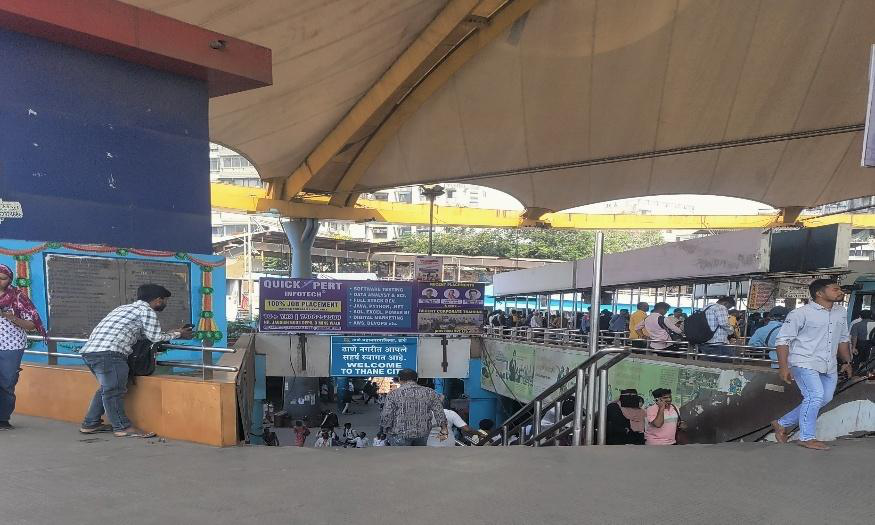
\includegraphics[width=0.75\textwidth]{fig_west_entry_deck.png}
\caption{Ground-level ``Welcome to Thane City'' entry deck, showing the staircase merge point
between the bus/auto stand and the station concourse.}
\end{figure}

\textbf{First-deck / skywalk entry (first-floor access).} The skywalk connected to the TMT depot
merges into the first-deck entrance of the station, used predominantly by bus commuters,
students, and pass-holders. Movement on the skywalk is smoother and faster than at ground level;
however, only two ticketing counters at deck level cause flow bifurcation: some commuters join
long queues at the deck counters, while others move downstairs back to the ground counters,
reversing flow direction. This reverse cross-movement between deck and ground-level users leads
to mid-path collisions, and the absence of signage or flow regulation causes natural breakdowns
in orderly movement.

\begin{figure}[H]
\centering
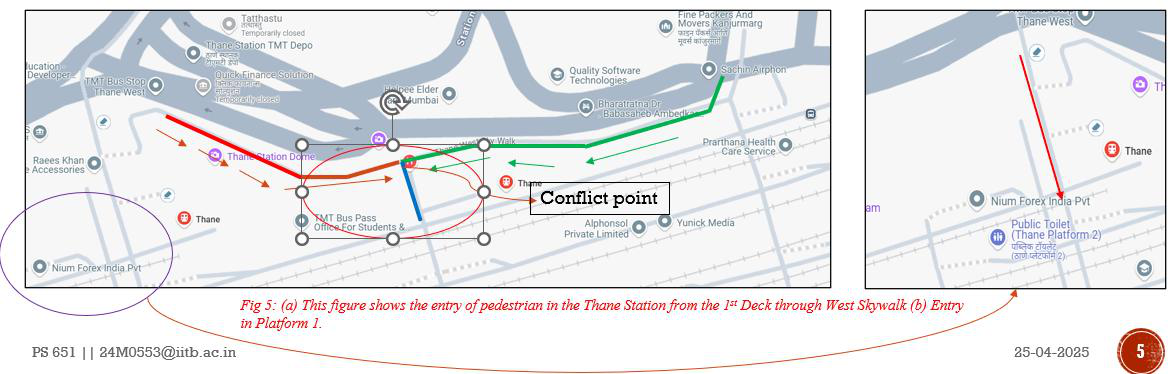
\includegraphics[width=0.85\textwidth]{fig_pedestrian_conflict.png}
\caption{Pedestrian flow diagram for the Thane West entry, showing entry from the first deck
through the West skywalk, entry to Platform~1, and the identified conflict point near the dome
staircase.}
\end{figure}

\textbf{Merge at the dome staircase to Platform 1.} A central staircase under the station dome
leads from the deck/ground levels to Platform~1. Passengers from both the deck and ground
converge at this single staircase, with no separate ``up'' and ``down'' sides established; heavy
bi-directional pushing occurs, especially during the morning peak (8--10~AM). The critical
conflict is that stair merging triggers shoulder pushing, queue breaking, and slow platform
clearance, with stair congestion often blocking the dome waiting area during high-density
periods.

\begin{figure}[H]
\centering
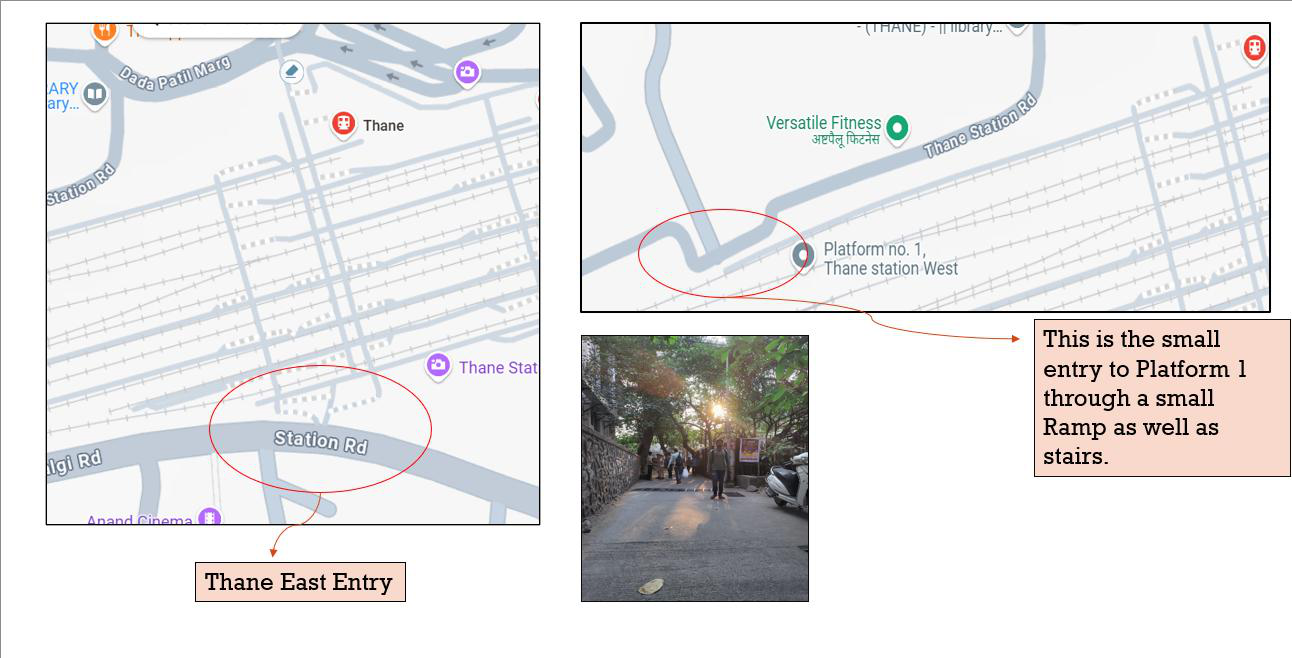
\includegraphics[width=0.75\textwidth]{fig_entry_points_map.png}
\caption{Additional station entries: the Thane East entry and the small ramp/stair entry to
Platform~1 on the West side.}
\end{figure}

\subsection{Conflict Zones and Risks}

Table~\ref{tab:conflictzones} summarises the principal pedestrian conflict zones identified
through field observation at the West entry.

\begin{table}[H]
\centering
\caption{Pedestrian conflict zones at the Thane West entry.}
\label{tab:conflictzones}
\small
\begin{tabular}{p{3.4cm}p{4.2cm}p{5.4cm}}
\toprule
\textbf{Location} & \textbf{Observed Behaviour} & \textbf{Associated Risk} \\
\midrule
Ground stair base & Pausing, clustering & Entry bottleneck, pushing \\
Skywalk junction & Flow reversal & Opposing-flow collision \\
Dome staircase & Stream merging & High density, panic trigger \\
Ticket counter turn & Sudden lateral switching & Trip/fall risk in a crowd \\
\bottomrule
\end{tabular}
\end{table}

\subsection{Parking System and Its Effect on Pedestrian Movement}

\textbf{Two-wheeler parking deck (first floor).} This is a structured, heavily used two-wheeler
deck above ground level. It becomes overcrowded by mid-morning, causing overflow onto walking
areas, and has no direct connection to platform entries; users must merge with the pedestrian
crowd below.

\textbf{Four-wheeler parking (east side).} Parking here is limited and loosely organised.
Vehicle circulation is difficult due to ongoing SATIS-East construction, and spillover parking
into pedestrian pathways has been observed.

\subsection{Key Observations from Mobility Behaviour}

\textbf{Mismatch between design and flow.} Station design elements, such as ticket counters and
stairs, do not match peak-hour volume patterns.

\textbf{Adaptive commuter behaviour.} Passengers exhibit reverse boarding from deck to ground
level and informal flow adjustment whenever formal systems break down.

\textbf{Lack of predictive flow management.} There is no dynamic flow zoning and no active crowd
dispersal announcements; static infrastructure forces commuters to self-manage congestion.

\textbf{Hidden risk factors.} Dome staircase congestion in particular represents a latent risk
for panic or stampede scenarios, underscoring the need for design interventions such as
separated up/down circulation and clearer wayfinding at the deck-to-ground transition.

\section{Thane Station as a People-Centric Mobility Hub: Broader Integration}

Beyond its internal systems, Thane railway station exists within a larger ecological,
infrastructural, and governance context that influences its operation and evolution.
Understanding these broader relationships is vital to appreciating Thane's role and the efforts
to make it a truly people-centric mobility hub in the Mumbai region.

\subsection{Urban and Infrastructural Ecosystem}

Thane station sits at the heart of Thane city, which has grown into a significant urban node
with a population of around 1.8~million. The station's presence has catalysed development in
its vicinity, a dense mix of markets, offices, and transit-oriented facilities surrounds it,
and the station effectively acts as a magnet for commuter activity, drawing residents from
adjoining areas such as Kalwa or Mumbra who travel to Thane to catch a fast train or a bus. This
has led to a web of connectivity: TMT, BEST, and NMMT buses converge at the station, integrating
three municipal bus systems, while auto-rickshaw stands on both sides ensure last-mile reach into
interior neighbourhoods. In the future, the under-construction Metro Line~4
(Wadala--Ghatkopar--Mulund--Thane--Kasarvadavali) will have a station near Thane railway station,
adding a north--south metro link to Mumbai. This multi-modal integration means Thane is not just
a railway stop but a city transportation hub where different modes interlink in a single
locality, improving accessibility and enhancing urban sustainability by encouraging public
transport use over private vehicles.

\begin{figure}[H]
\centering
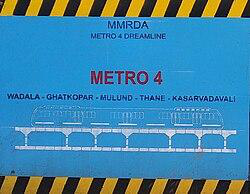
\includegraphics[width=0.5\textwidth]{fig_metro4_signboard.png}
\caption{Metro Line~4 (Wadala--Ghatkopar--Mulund--Thane--Kasarvadavali) signage.}
\end{figure}

This confluence also creates stresses: the roads outside Thane station, especially on the West,
face chronic traffic congestion due to the sheer volume of buses, autos, and drop-offs. The
Station Area Traffic Improvement Scheme (SATIS), implemented by the Thane Municipal
Corporation, aimed to untangle this by constructing the elevated deck for buses and autos and
creating segregated lanes. SATIS-West (completed around 2010) alleviated some street-level chaos
by moving much of it onto the elevated bus depot and skywalks. SATIS-East is now underway,
including an elevated deck and a new 11-storey multi-modal tower on the East side, a joint
venture of the Rail Land Development Authority and TMC, providing parking, a bus terminus, and
commercial spaces integrated with the eastern side of the station. The goal is to mirror the
West's functionality, balancing flows by attracting more people to the East entrance while also
generating revenue through retail and offices in the tower that can fund station improvements.
By 2026, when SATIS-East is slated for completion, Thane station's infrastructure ecosystem will
include a modern concourse, better dispersal areas, and direct links to city roads, embodying a
transit-oriented development model that integrates land use with transit infrastructure.

The station also interacts with the city in environmental terms. Large footfalls mean issues
like waste management become significant: TMC and the railways coordinate to clean up garbage,
such as the dry waste that caused the March~2025 platform fire. Noise and vehicular emissions
around the station affect urban air quality, but conversely, every commuter who takes a train or
bus from Thane instead of driving reduces car usage. In this sense, Thane station is a
sustainability asset for the region, moving nearly 7~lakh people by rail daily and thereby
lowering overall congestion and pollution in the metro area.

\subsection{Governance and Management Collaboration}

Thane station's effective functioning requires coordination between multiple governance
entities: primarily Indian Railways, which owns and operates the station and trains, and the
Thane Municipal Corporation, which manages the city infrastructure around it. This interplay has
seen both successes and frictions. The FOB reconstruction is one example of collaboration: TMC
funded and built some bridges to help residents cross the railway, and when these became unsafe,
it worked with the Railways to rebuild them. The new SATIS-East tower is being jointly developed,
aligning the railway's revenue plans with the city's urban plan. Another governance aspect is
security: RPF (under the Ministry of Railways) and GRP (under the state Home Department) share
jurisdiction, requiring coordination; Thane has a good RPF--GRP cooperation model, conducting
joint drills and sharing duties in crises, though passengers can sometimes fall in the cracks of
jurisdiction for issues like petty crime outside the station boundary.

The people-centric focus in governance is visible through passenger associations and public
feedback channels. Commuter groups in Thane voice concerns to railway officials and municipal
authorities, which has led to tangible improvements such as additional train services and quick
fixes for malfunctioning indicators or dirty platforms, aided by real-time social-media
monitoring by authorities. A broader governance initiative to decongest Thane is the proposal to
construct a new suburban railway station between Thane and Mulund (at Kopri), led jointly by TMC
and the railways, aiming to redistribute passenger load by creating an alternate stop and access
point for Thane city, indicating forward-thinking governance that recognises the need for new
capacity alongside managing the existing station.

In summary, Thane Station's mobility ecology cannot be divorced from its urban and governance
context. Its success as a people-centric hub results from integrated planning, blending
infrastructure (skywalks, depots, footbridges) with operational management, and involving
stakeholders from government bodies to citizen groups. The station is a microcosm of the city:
dynamic, crowded, occasionally chaotic, but constantly adapting through both top-down
interventions and bottom-up user behaviours.

\section{Conclusion and Recommendations}

The mobility ecology of Thane Railway Station is an intricate tapestry of infrastructure, human
behaviour, technology, and institutional management. Through the analysis of the Passenger
Management, Emergency/Disaster Management, and Technology Integration systems via the
Hardware--Software--Practice framework, several key themes emerge.

\textbf{Interdependence of systems.} Improvements or failings in one system affect the others.
Better passenger management (additional FOBs, disciplined queues) directly reduces the
likelihood of emergencies such as stampedes; robust technology (CCTV, announcements) enhances
daily management and emergency response by providing information and oversight. The three
systems function as subsystems of a larger organism, the station, and must be developed in
tandem.

\textbf{People-centric design and operations.} Thane station exemplifies both the power and the
challenge of people-centric design. Integrating bus terminals and skywalks has made the station
extremely convenient for mode interchange, but overlooking human factors, such as the need for
separate entry/exit flows or sufficient waiting space, has led to discomfort and safety
hazards. The lesson is that hardware must be designed with human behaviour in mind: wide
pathways, clear signage, and universal accessibility are not optional in such a busy hub, and
continued audits of how people actually use (or struggle with) the station should inform future
design tweaks.

\textbf{Resilience and adaptation.} The daily handling of 6--8~lakh passengers is a testament to
operational resilience, with staff and commuters co-creating adaptive practices that keep the
system running even under strain. However, resilience has limits: the station is operating near
capacity, and further ridership growth or unexpected surges could overwhelm it. Building
redundancy and a buffer, such as more footbridges than the bare minimum, emergency exits, and
backup power and communication, is essential to handle worst-case scenarios; the upcoming SATIS-East and
new substation will provide much-needed capacity and fallback options.

\textbf{Safety and comfort as priorities.} From a commuter's perspective, the paramount concerns
are safety (from crime, accidents, or being trampled) and comfort (accessibility for all
ages/abilities, cleanliness, and order). A recommended \textbf{Comprehensive Crowd Management
Plan} for Thane could include deploying more personnel at peak hours, using PA announcements to
direct flows, marking bi-directional lanes on bridges, and enforcing queueing at platforms beyond
just the ladies' coaches, drawing on practices from other busy global hubs such as floor
markings for orderly boarding.

\textbf{Enhancing emergency preparedness.} Installing basic security screening (even handheld
metal detectors at peak hours), ensuring 24/7 medical assistance (reviving a ``one-rupee clinic''
model or tying up with hospitals for round-the-clock paramedics), conducting regular mock drills
including passengers where feasible, and developing a formal monsoon action plan would all
strengthen the station's readiness for both routine and large-scale emergencies.

\textbf{Leveraging technology further.} Thane can pilot AI-based crowd density monitoring that
triggers automated alerts when a FOB nears capacity, smartphone notifications on less-crowded
exits, and unified ticketing across train, bus, and metro. Continued investment in reliable,
accurate information systems and extended Wi-Fi coverage across the station and adjacent bus
stops would further enhance user comfort.

\textbf{Governance and continuous improvement.} Sustained political and administrative attention
to Thane, a high-profile suburban station, must continue in a data-driven manner: footfall
counters at entries, feedback kiosks or periodic satisfaction surveys, and a quarterly
station-level committee of railway officials, local government representatives, and commuter
representatives to close the governance feedback loop. Planned capacity additions, such as the
proposed satellite station at Kopri, should be fast-tracked to relieve pressure on Thane.

In conclusion, Thane Railway Station stands as a vital, living system at the core of Mumbai's
transit network, showcasing how hardware, software, and practice coalesce to either create a
seamless mobility experience or, if not optimally aligned, lead to friction and risk. The
station has many strengths, such as high connectivity, continuous upgrades, and dedicated staff,
but also pressing challenges in crowd management and safety that need redressal. By implementing
holistic improvements across physical design, management strategies, and technological tools,
and by strengthening the partnership between the station and the city, Thane can become a model
people-centric mobility hub: accessible, safe, and comfortable for all, while efficiently
handling the demands of a growing urban populace.

\begin{thebibliography}{10}

\bibitem{interview}
Station Manager Interview and Responses: \textit{Thane Station Infrastructure \& Operations
Details}, field interview conducted as part of this study, 2025.

\bibitem{ht2023}
Hindustan Times (2023). \textit{Overcrowding at Thane railway station raises concerns of poor
crowd management}. Mumbai news, Hindustan Times.

\bibitem{toi2013}
Times of India (2013). \textit{Thane is busiest railway station in Mumbai}: MRVC Survey Data.
Mumbai News, The Times of India.

\bibitem{toi2024fob}
Times of India (2024). \textit{Now, 2 crucial FOBs ready to use at Thane railway stn}:
Infrastructure Upgrade Report. Thane News, The Times of India.

\bibitem{toi2025fire}
Times of India (2025). \textit{Minor fire at Thane station halts two local services briefly}:
Incident Report. Thane News, The Times of India.

\bibitem{ht2018bomb}
Hindustan Times (2018). \textit{Suspicious bag triggers bomb scare near Thane railway station}.
Mumbai news, Hindustan Times.

\bibitem{mm2018queue}
Mumbai Mirror (2018). \textit{Local train queue system finds many takers}: Commuter Behaviour,
Western Railway (WR): From Andheri to Thane.

\bibitem{jugyah2023}
Jugyah.com (2023). \textit{Thane Railway Station: In-Depth Guide}: Station Facilities \&
Connectivity.

\bibitem{toi2025satis}
Times of India (2025). \textit{Thane station to host 11-storey tower for retail space, offices,
hotels}: SATIS-East Development. Thane News, The Times of India.

\bibitem{elets2018}
Elets eGov Magazine (2018). \textit{Thane's Transformation into a Smart City}: City
Initiatives (Sunil Chavan Interview).

\end{thebibliography}

\end{document}
